\documentclass{beamer}
\graphicspath{{assets}}

%Information to be included in the title page:
\title{PRICO, an AI Powered E-Commerce Platform}
\subtitle{Senior Capstone Research Project}
\institute{Addis Ababa Science and Technology University}
\date{2025}


\begin{document}

\frame{\titlepage}

\begin{frame}
	\frametitle{General Objectives}

	Our general objective is to develop an AI-powered e-commerce platform. With enhanced user
	engagement through personalized product recommendations, efficient scanning features, and
	reliable payment and delivery integrations.
\end{frame}

\begin{frame}
	\frametitle{Specific Objectives}
	\begin{itemize}
		\item Requirement Gathering
		\item System Design and Architecture
		\item AI-Based Recommendation Engine
		\item Feature Development
		\item Vendor Verification System
		\item Scalability and Security Enhancements
		\item Testing and Quality Assurance
		\item User Training and Documentation
		\item Deployment
		\item Post-Deployment Support and Maintenance
	\end{itemize}
\end{frame}

\begin{frame}
	\frametitle{Project Scope}
	The scope of this study includes developing a functional prototype of our app
	(PRICO) that incorporates AI-driven features, barcode scanning tools, Chapa
	payment integration, and delivery services.
\end{frame}

\begin{frame}
	\frametitle{Project Scope}
	\framesubtitle{Focus Areas}
	\begin{itemize}
		\item \textbf{AI Features}: Personalized recommendations with continuous learning.
		\item \textbf{Vendor Verification}: Ensure legitimate sellers and reduce fraud.
		\item \textbf{Barcode Tools}: "Scan to Post" for sellers, "Scan to Find" for buyers.
		\item \textbf{Payment Integration}: Secure Chapa gateway with multi-payment support.
		\item \textbf{Delivery Services}: Real-time tracking and buyer notifications.
		\item \textbf{Reels-Like Videos}: Short product videos and AI-driven trending insights.
	\end{itemize}
\end{frame}

\begin{frame}
	\frametitle{Methodology}
	\framesubtitle{Overview}
	Development Model: Incremental Development Model
	\begin{itemize}
		\item Iterative development with continuous feedback.
		\item Deliver functional modules in manageable stages.
	\end{itemize}
\end{frame}

\begin{frame}
	\frametitle{Methodology}
	\framesubtitle{Requirement Gathering}
	\begin{itemize}
		\item \textbf{Objective}: Understand buyer and seller needs.
		\item \textbf{Methods}:
		      \begin{itemize}
			      \item \textbf{Surveys}: Scalable quantitative data collection.
			      \item \textbf{Interviews}: In-depth qualitative insights.
		      \end{itemize}
		\item \textbf{Benefits}: Comprehensive understanding of user requirements.
	\end{itemize}
\end{frame}

\begin{frame}
	\frametitle{Methodology}
	\framesubtitle{Requirement Analysis}
	\begin{itemize}
		\item \textbf{Tools}: Object-Oriented Analysis (OOA) and Unified Modeling Language
		      (UML).
		\item \textbf{Deliverables}:
		      \begin{itemize}
			      \item Use-case diagrams
			      \item Class diagrams
			      \item Deployment diagrams
		      \end{itemize}
		\item \textbf{Purpose}: Translate user requirements into clear system designs.
	\end{itemize}
\end{frame}

\begin{frame}
	\frametitle{Methodology}
	\framesubtitle{System Design}
	\begin{itemize}
		\item \textbf{UI/UX Design Tool}: Figma
		      \begin{itemize}
			      \item Collaborative features for real-time feedback.
		      \end{itemize}
		\item \textbf{Deliverables}:
		      \begin{itemize}
			      \item High-fidelity prototypes
			      \item User journey wireframes
		      \end{itemize}
	\end{itemize}
\end{frame}

\begin{frame}
	\frametitle{Methodology}
	\framesubtitle{Implementation}
	Approach: Incremental development of key modules:
	\begin{itemize}
		\item AI recommendation engine
		\item Barcode scanning
		\item Chapa payment integration
		\item Delivery tracking
		\item \textbf{Technologies}
		      \begin{itemize}
			      \item Mobile: Flutter
			      \item Web: React
			      \item Backend: Go
		      \end{itemize}
		\item \textbf{Architecture}: Monolithic with external services.
	\end{itemize}
\end{frame}

\begin{frame}
	\frametitle{Methodology}
	\framesubtitle{Testing}
	\textbf{Testing Methods}:
	\begin{itemize}
		\item \textbf{Unit Testing}: Validate individual components.
		\item \textbf{Automated Testing}:
		      \begin{itemize}
			      \item Selenium for web apps.
			      \item Appium for mobile apps.
			      \item Postman/Bruno for API testing.
		      \end{itemize}
		\item \textbf{Performance Testing}:
		      \begin{itemize}
			      \item Tools: JMeter for load testing.
			      \item Focus: Scalability and resilience.
		      \end{itemize}
	\end{itemize}
\end{frame}

\begin{frame}
	\frametitle{Methodology}
	\framesubtitle{Deployment}
	\begin{itemize}
		\item \textbf{Hosting}: Cloud-based solutions (Hahu Cloud, Yegara Host, Telecloud).
		\item \textbf{Deployment Tools}: Docker for consistency across environments.
		\item \textbf{Focus}: Scalable, secure, and reliable hosting.
	\end{itemize}
\end{frame}

\begin{frame}
	\frametitle{Plan of Activities}
	\framesubtitle{Overview}
	\begin{itemize}
		\item \textbf{Timeline}: November to May
		\item \textbf{Phases}: Project definition, development, integration, testing, deployment, and defense.
		\item \textbf{Goal}: Deliver a functional, scalable, and user-focused app (PRICO).
	\end{itemize}
\end{frame}

\begin{frame}
	\frametitle{Feasibility study}
	\framesubtitle{Technical Feasibility}
	\begin{itemize}
		\item \textbf{Impact}: Uses modern, well-documented tools (Flutter, React, Go). Expertise required.
		\item \textbf{Verdict}: Technically feasible with accessible tools and skilled team.
	\end{itemize}
\end{frame}

\begin{frame}
	\frametitle{Feasibility study}
	\framesubtitle{Technical Feasibility}
	\begin{itemize}
		\item \textbf{Impact}: Uses modern, well-documented tools (Flutter, React, Go). Expertise required.
		\item \textbf{Verdict}: Technically feasible with accessible tools and skilled team.
	\end{itemize}
\end{frame}

\begin{frame}
	\frametitle{Feasibility study}
	\framesubtitle{Operational Feasibility}
	\begin{itemize}
		\item \textbf{Impact}: Operational requirements (fraud prevention, AI recommendations, secure payments, vendor verification, delivery tracking) align with project goasl
		\item \textbf{Verdict}: Operationally feasible with team capabilities and aligned objectives.
	\end{itemize}
\end{frame}

\begin{frame}
	\frametitle{Feasibility study}
	\framesubtitle{Economic Feasibility}
	\begin{itemize}
		\item \textbf{Impact}: Budget of ~4,000 ETB is affordable. Potential revenue offsets costs.
		\item \textbf{Verdict}: Economically feasible with sustainable financial returns.
	\end{itemize}
\end{frame}

\begin{frame}
	\frametitle{Feasibility study}
	\framesubtitle{Legal Feasibility }
	\begin{itemize}
		\item\textbf{Impact}: Requires compliance with data protection, e-commerce, and payment regulations.
		\item\textbf{Verdict}: Legally feasible if regulatory standards are met.
	\end{itemize}
\end{frame}

\begin{frame}
	\frametitle{Feasibility study}
	\framesubtitle{Time Feasibility}
	\begin{itemize}
		\item\textbf{Impact}: Six-month timeline. Incremental approach minimizes risks.
		\item\textbf{Verdict}: Time feasible with realistic schedule and management.
	\end{itemize}
\end{frame}

\begin{frame}
	\frametitle{Feasibility study}
	\framesubtitle{Environmental Feasibility}
	\begin{itemize}
		\item\textbf{Impact}: Minimal environmental footprint with energy-efficient hosting and digital receipts.
		\item\textbf{Verdict}: Environmentally feasible.
	\end{itemize}
\end{frame}

\begin{frame}
	\frametitle{Feasibility study}
	\framesubtitle{Social Feasibility}
	\begin{itemize}
		\item\textbf{Impact}: Promotes trust in e-commerce, supports local vendors, and improves user experience.
		\item\textbf{Verdict}: Socially feasible with significant positive impact.
	\end{itemize}
\end{frame}

\begin{frame}
	\frametitle{Significance of the Study}
	\textbf{User Benefits}:
	\begin{itemize}
		\item AI-powered product recommendations for personalized shopping.
		\item Secure Chapa payments and vendor verification to prevent fraud.
		\item Streamlined features ensure a user-friendly and efficient experience.
	\end{itemize}
	\textbf{Seller Empowerment}
	\begin{itemize}
		\item Tools like “Scan to Post” and video showcases enhance visibility.
		\item Drives economic growth for local businesses.
	\end{itemize}
\end{frame}

\begin{frame}
	\frametitle{Significance of the Study (Cont'd)}
	\textbf{Market Impact}:
	\begin{itemize}
		\item Fills gaps in Ethiopian e-commerce with secure, trusted platforms.
		\item Boosts SMEs by reducing costs and increasing market access (+45%).
		\item Builds consumer trust, increasing sales by up to 70%.
	\end{itemize}
	\textbf{Contribution}
	\begin{itemize}
		\item Enhances the region's economic and technological development.
	\end{itemize}
\end{frame}

\begin{frame}
	\frametitle{Literature Review}
	\framesubtitle{Overview}
	\begin{itemize}
		\item\textbf{Purpose}: Contextualizes the study, identifies gaps, and charts a path forward.
		\item\textbf{Focus}: AI's transformative role in e-commerce and localized solutions for Ethiopia.
		\item\textbf{Objective}: Position PRICO as a scalable, innovative solution for the Ethiopian e-commerce market.
	\end{itemize}
\end{frame}

\begin{frame}
	\frametitle{Literature Review}
	\framesubtitle{AI for Personalized Recommendations}
	\begin{itemize}
		\item \textbf{Study}: Smith et al.
		\item \textbf{Methodology}: Collaborative filtering + deep learning (1M+ user interactions).
		\item \textbf{Results}:
		      \begin{itemize}
			      \item 30\% ↑ purchase rates.
			      \item 15\% ↓ customer churn.
			      \item Deep learning handles sparse data well.
		      \end{itemize}
		\item \textbf{Limitation}: Resource-intensive models
	\end{itemize}
\end{frame}

\begin{frame}
	\frametitle{Literature Review}
	\framesubtitle{Barcode and QR Code Scanning in Retail}
	\begin{itemize}
		\item \textbf{Study}: Jones et al. [18]
		\item \textbf{Prototype}: Barcode/QR scanning for product listing & info retrieval.
		\item \textbf{Results}:
		      \begin{itemize}
			      \item 40\% ↓ manual errors.
			      \item 25\% ↑ buyer satisfaction.
			      \item Improved inventory management.
		      \end{itemize}
		\item \textbf{Challenges}: Requires robust mobile infrastructure.
	\end{itemize}
\end{frame}

\begin{frame}
	\frametitle{Literature Review}
	\framesubtitle{AI in Payment \& Delivery Systems}
	\begin{itemize}
		\item \textbf{Study}: Lee et al. [19]
		\item \textbf{Framework}: Optimized payment gateways + AI-based dynamic delivery routes.
		\item \textbf{Results}:
		      \begin{itemize}
			      \item 20\% ↓ transaction time.
			      \item 15\% ↑ delivery efficiency.
			      \item 10\% ↑ customer retention.
		      \end{itemize}
		\item \textbf{Challenges}: Needs strong data infrastructure.
	\end{itemize}
\end{frame}

\begin{frame}
	\frametitle{Literature Review}
	\framesubtitle{Short-Form Video Promotion for E-Commerce}
	\begin{itemize}
		\item \textbf{Study}: Chen et al. [20]
		\item \textbf{System}: Swipe-based short-form video for product showcases (15–60 secs).
		\item \textbf{Results}:
		      \begin{itemize}
			      \item 50\% ↑ engagement rates.
			      \item 35\% ↑ conversions for visually dynamic products.
		      \end{itemize}
		\item \textbf{Challenges}: Video compression and content moderation needed.
	\end{itemize}
\end{frame}

\begin{frame}
	\frametitle{Literature Review}
	\framesubtitle{Global and Local Platform Insights}
	\begin{itemize}
		\item \textbf{Amazon}: AI-driven logistics & recommendations; resource-intensive.
		\item \textbf{Jumia}: Cash-on-delivery adapted for Africa; lacks scalability.
		\item \textbf{Alibaba}: Advanced tools empower SMEs; complex for smaller markets.
		\item \textbf{Zmall}: Focus on delivery services; lacks personalization.
	\end{itemize}
	So what do we plan to do about it?
	\begin{itemize}
		\item PRICO aims to brigde gaps between global capabilities and local needs.
	\end{itemize}
\end{frame}

\begin{frame}
	\frametitle{Identifying Gaps}
	\begin{itemize}
		\item \textbf{Limited Personalization}: No AI-driven engagement on Ethiopian platforms.
		\item \textbf{Scalability Issues}: Reliance on manual processes.
		\item \textbf{Fragmented Systems}: Payment, delivery, and discovery not integrated.
		\item \textbf{Weak Trust Mechanisms}: Inadequate vendor verification.
		\item \textbf{Lack of Modern Formats}: No short-form video for dynamic user interaction.
	\end{itemize}
\end{frame}

\begin{frame}
	\frametitle{Lessons Learned}
	\begin{itemize}
		\item \textbf{Personalization}: AI improves engagement and vendor visibility.
		\item \textbf{Localization}: Tailored features (e.g., Telebirr) drive adoption.
		\item \textbf{Trust}: Verified sellers and secure payments build user confidence.
		\item \textbf{Automation}: Barcode scanning & dynamic routing reduce inefficiencies.
		\item \textbf{Innovative Formats}: Short-form videos increase conversions.
	\end{itemize}
\end{frame}

\begin{frame}
	\frametitle{PRICO’s Positioning}
	\begin{itemize}
		\item \textbf{Goal}: Redefine Ethiopian e-commerce with a scalable, AI-driven platform.
		\item \textbf{Approach}: Bridge global best practices and local market needs.
		\item \textbf{Next Steps}: Problem analysis and architecture modeling.
	\end{itemize}
\end{frame}

\begin{frame}
	\frametitle{Existing System and Its Problems}
	\framesubtitle{Ashewa}
	\begin{itemize}
		\item \textbf{Strengths}: localized approach, integrated payment and
		      seller tools
		\item \textbf{Weaknesses}: no transparency in delivery methods and
		      vendor verification, personalized recommendations
		\item \textbf{Opportunities}: integrating AI recommendations, vendor
		      verification, streamlined delivery
		\item \textbf{Threats}: competition from advanced platforms, both
		      locally and globally
	\end{itemize}
\end{frame}

\begin{frame}
	\frametitle{Existing System and Its Problems}
	\framesubtitle{Jiji}
	\begin{itemize}
		\item \textbf{Strengths}: straightforward tools for listing products
		      services
		\item \textbf{Weaknesses}: lack of vendor verification, personalized
		      recommendations
		\item \textbf{Opportunities}: implementing vendor verification, fraud
		      detection, recommendations
		\item \textbf{Threats}: security concerns and limited features may
		      drive users to other platforms
	\end{itemize}
\end{frame}

\begin{frame}
	\frametitle{Existing System and Its Problems}
	\framesubtitle{Amazon}
	\begin{itemize}
		\item \textbf{Strengths}: best in class recommendation, delivery, and
		      payment systems
		\item \textbf{Weaknesses}: high shipping costs, delivery times and
		      customs issues for Ethiopian users
		\item \textbf{Opportunities}: adapting to local needs by regional
		      payment options and language support
		\item \textbf{Threats}: platforms inability to address local needs
		      leaves room for competitors
	\end{itemize}
\end{frame}

\begin{frame}
	\frametitle{Existing System and Its Problems}
	\framesubtitle{AliExpress}
	\begin{itemize}
		\item \textbf{Strengths}: affordable prcing, global shipping options,
		      frequent sales
		\item \textbf{Weaknesses}: long delivery times, high customs duties,
		      inconsistent product quality for Ethiopian users
		\item \textbf{Opportunities}: faster shipping, better QA, localization
		\item \textbf{Threats}: delays and quality issues may drive users away
	\end{itemize}
\end{frame}

\begin{frame}
	\frametitle{Specifying the Requirements of the Proposed Solution}
	\framesubtitle{}
	To address limitations of existing platforms like Ashewa and Jiji, a detailed
	survey of buyers and sellers was conducted. Key findings included:
	\begin{itemize}
		\item \textbf{Buyers' Pain Points}: Lack of trust mechanisms, inefficient product search, and inadequate personalized recommendations.
		\item \textbf{Sellers' Challenges}: Limited promotional tools, absence of analytics, and delivery issues.
	\end{itemize}
\end{frame}

\begin{frame}
	\frametitle{Specifying the Requirements of the Proposed Solution}
	\framesubtitle{Proposed Features}
	Based on the survey results, we've arrived at the following required
	functional requirements for the platform:
	\begin{itemize}
		\item Vendor verification to enhance trust.
		\item Short-form video promotions for dynamic product showcases.
		\item Automated updates and advanced search filters.
		\item Social shopping features like "What’s my friend buying?"
	\end{itemize}
\end{frame}

\begin{frame}
	\frametitle{Specifying the Requirements of the Proposed Solution}
	\framesubtitle{Non-Functional Insights}
	\begin{itemize}
		\item Local language support (e.g., Amharic).
		\item Integration with local payment methods (e.g., Telebirr).
		\item Scalability to accommodate growth and personalized features.
	\end{itemize}
\end{frame}

\begin{frame}
	\frametitle{Functional Requirements}
	\framesubtitle{}
	\begin{itemize}
		\item User Registration And Authentication
		\item User Account Management
		\item Vendor Registration and Verification
		\item AI Based Recommendation Engine
		\item Short Form Videos for Product Promotion
		\item Fully Featured Product Search Engine
		\item Delivery Mechanisms
		\item Barcode Based Product Registrations
		\item Integration With Payment Systems
		\item Vendors Dashboard and Analytics
		\item Vendor/Product Reporting
		\item Basic Social Features
	\end{itemize}
\end{frame}

\begin{frame}
	\frametitle{Non-Functional Requirements}
	\framesubtitle{Availability}
	For this system, we aim for 99\% SLA. To achieve that, the following
	are implemented:
	\begin{itemize}
		\item Stateless App Servers
		\item Redundant Infrastructure
		\item Failover Systems
		\item Real-Time Monitoring
	\end{itemize}
\end{frame}

\begin{frame}
	\frametitle{Non-Functional Requirements}
	\framesubtitle{Performance}
	\begin{itemize}
		\item \textbf{Response Time Goals}: Targeting a median response time of 500ms and a 99th
		      percentile of no more than 2 seconds
		\item Efficient Media Processing
		\item Load Balancing
		\item Optimizing queries and caching
	\end{itemize}
\end{frame}

\begin{frame}
	\frametitle{Non-Functional Requirements}
	\framesubtitle{Accessibility and Localization}
	\begin{itemize}
		\item \textbf{Initial Language Support}: Amharic and English at launch,
		      with more to come later
		\item Localized Payment Integration
		\item Responsive Design
		\item User-Centric Navigation
	\end{itemize}
\end{frame}

\begin{frame}
	\frametitle{Non-Functional Requirements}
	\framesubtitle{Security}
	\begin{itemize}
		\item Data encryption
		\item TLS everywhere
		\item Password hashing
		\item Stateless token authentication
		\item Regular security audits
	\end{itemize}
\end{frame}

\begin{frame}
	\frametitle{System Architecture}
	\framesubtitle{}
	\textbf{Design Principles}: Simplicity, scalability, and extensibility tailored to
	Ethiopia’s unique market.

	Core Structure:
	\begin{itemize}
		\item \textbf{Monolithic Architecture}: Centralized application logic for ease of development and deployment.
		\item \textbf{External Services}: Specialized services for resource-intensive or isolated tasks to ensure flexibility and scalability.
	\end{itemize}
\end{frame}

\begin{frame}
	\frametitle{System Architecture}
	\framesubtitle{Deployment Diagram}
	\begin{figure}
		\begin{center}
			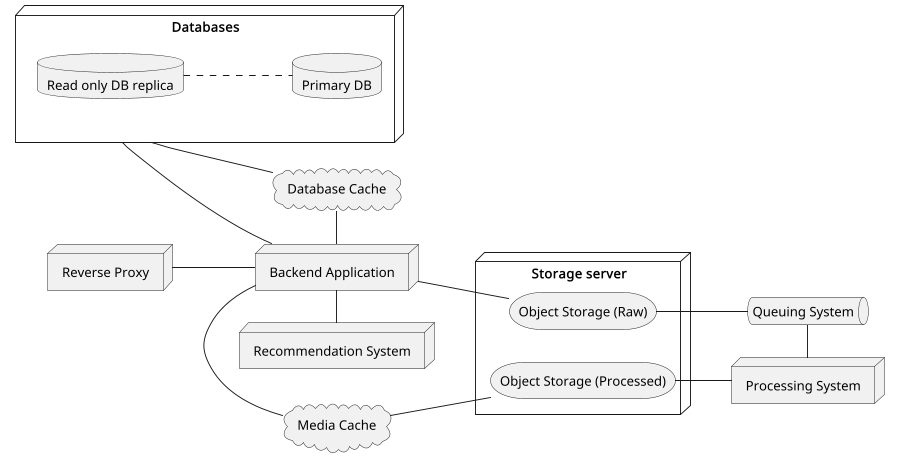
\includegraphics[width=0.95\textwidth]{diagrams/deployment}
		\end{center}
		\caption{Deployment Diagram for PRICO}\label{fig:fig1}
	\end{figure}
\end{frame}

\begin{frame}
	\frametitle{System Architecture}
	\framesubtitle{High-Level Components}
	\begin{itemize}
		\item Reverse Proxy
		\item Backend Application
		\item Recommendation System
		\item Storage Server
		      \begin{itemize}
			      \item Object Storage (Raw)
			      \item Object Storage (Processed)
		      \end{itemize}
		\item Processing System
		      \begin{itemize}
			      \item Queuing System
		      \end{itemize}
		\item Media Cache
		\item Databases
		      \begin{itemize}
			      \item Database Cache
		      \end{itemize}
	\end{itemize}
\end{frame}

\begin{frame}
	\frametitle{System Architecture}
	\framesubtitle{Interactions Between Components}
	\begin{itemize}
		\item Request Flow
		\item Media Handling
		\item Recommendation Delivery
	\end{itemize}
\end{frame}

\begin{frame}
	\frametitle{System Architecture}
	\framesubtitle{Scalability, Maintainability, and Extensibility of the Architecture}
	Scalability:
	\begin{itemize}
		\item Stateless backend enables horizontal scaling.
		\item Read-only database replica and caching layers handle high read workloads.
		\item Queuing system manages resource-intensive tasks like media processing.
	\end{itemize}
	Modularity:
	\begin{itemize}
		\item Monolithic backend centralizes core logic, simplifying development and debugging.
		\item External services (e.g., recommendation engine, media processing) are independently maintainable and replaceable.
		\item Extensible design supports features like advanced AI models or third-party integrations.
	\end{itemize}
\end{frame}

\begin{frame}
	\frametitle{Use Case Modeling}
	\framesubtitle{Actors}
	\begin{enumerate}
		\item Buyer
		\item Seller
		\item Admin
		\item Delivery Agent
	\end{enumerate}
\end{frame}

\begin{frame}
	\frametitle{Use Case Modeling}
	\framesubtitle{Use Case Diagram}
	\begin{figure}
		\begin{center}
			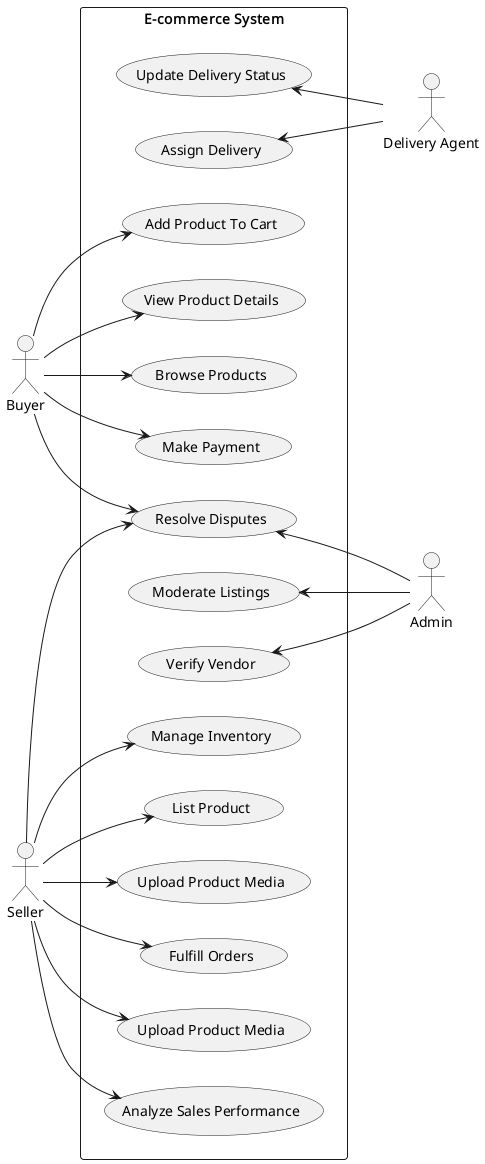
\includegraphics[width=0.25\textwidth]{diagrams/use-case}
		\end{center}
		\caption{Use Case Diagram for PRICO}\label{fig:fig1}
	\end{figure}
\end{frame}

\begin{frame}
	\frametitle{Object Modeling}
	\framesubtitle{Class Diagram}
	\begin{figure}
		\begin{center}
			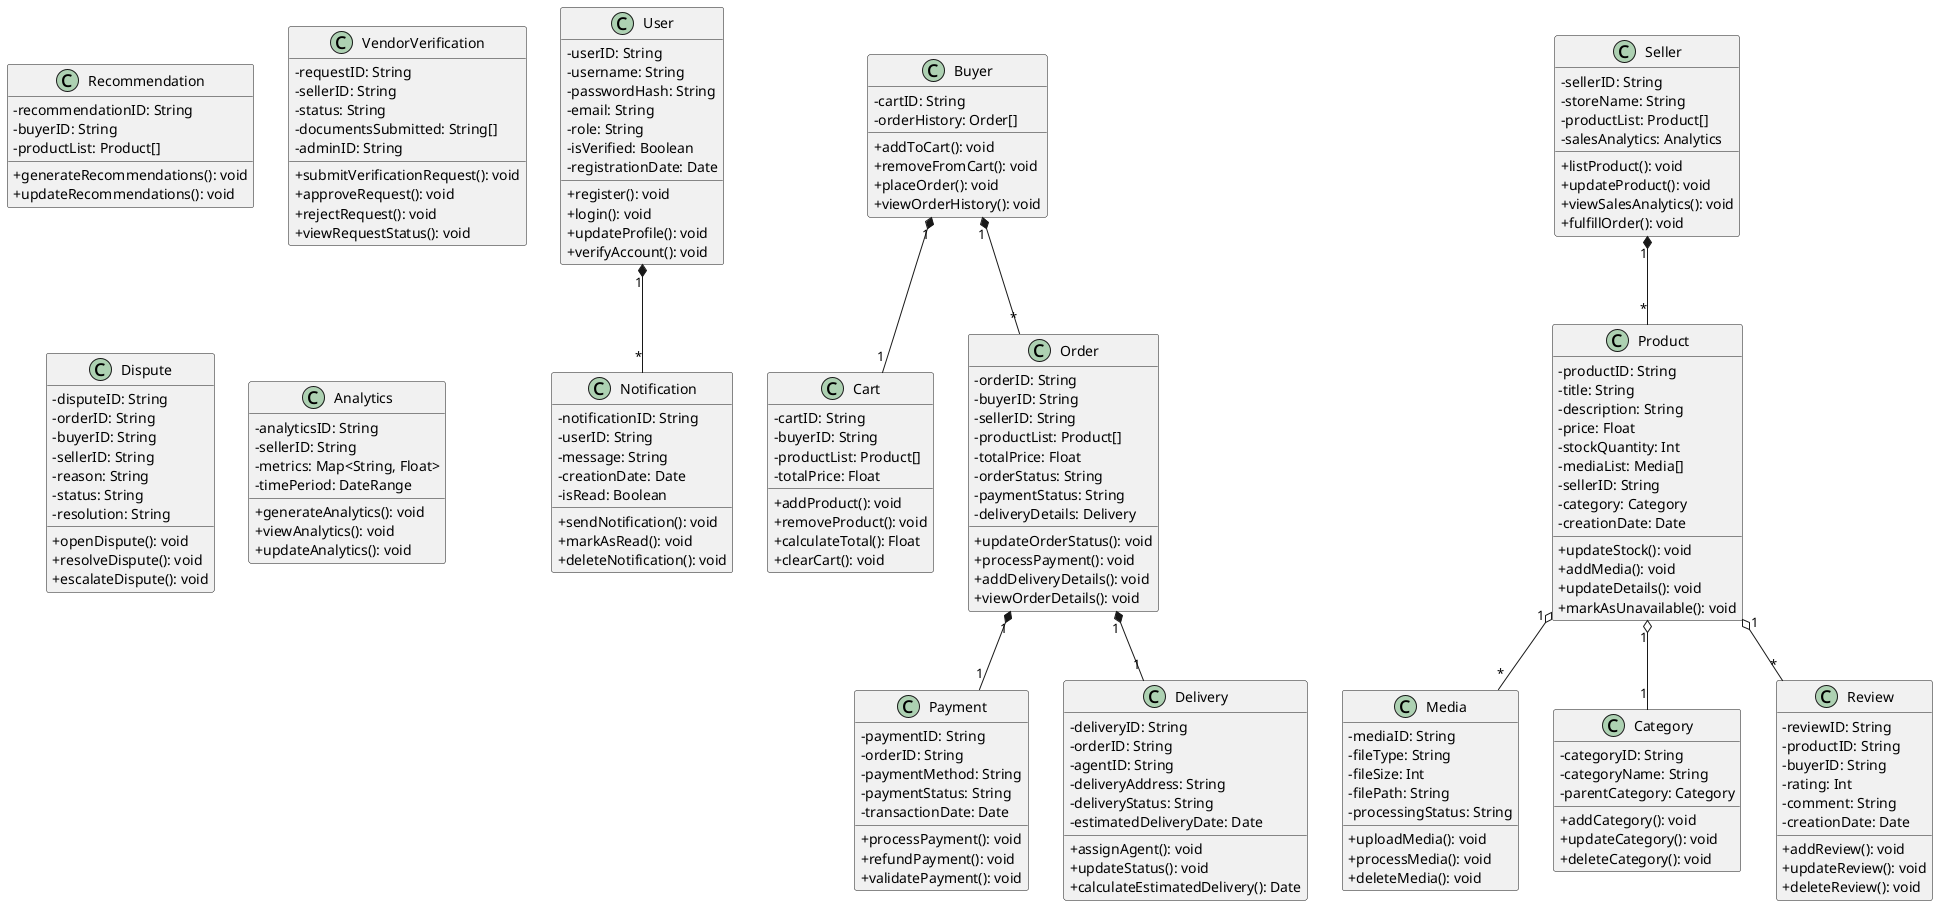
\includegraphics[width=1\textwidth]{diagrams/class}
		\end{center}
		\caption{Class Diagram for PRICO}\label{fig:fig2}
	\end{figure}
\end{frame}

\begin{frame}
	\frametitle{Database Modeling}
	\framesubtitle{Entity-Relationship Diagram}
	\begin{figure}
		\begin{center}
			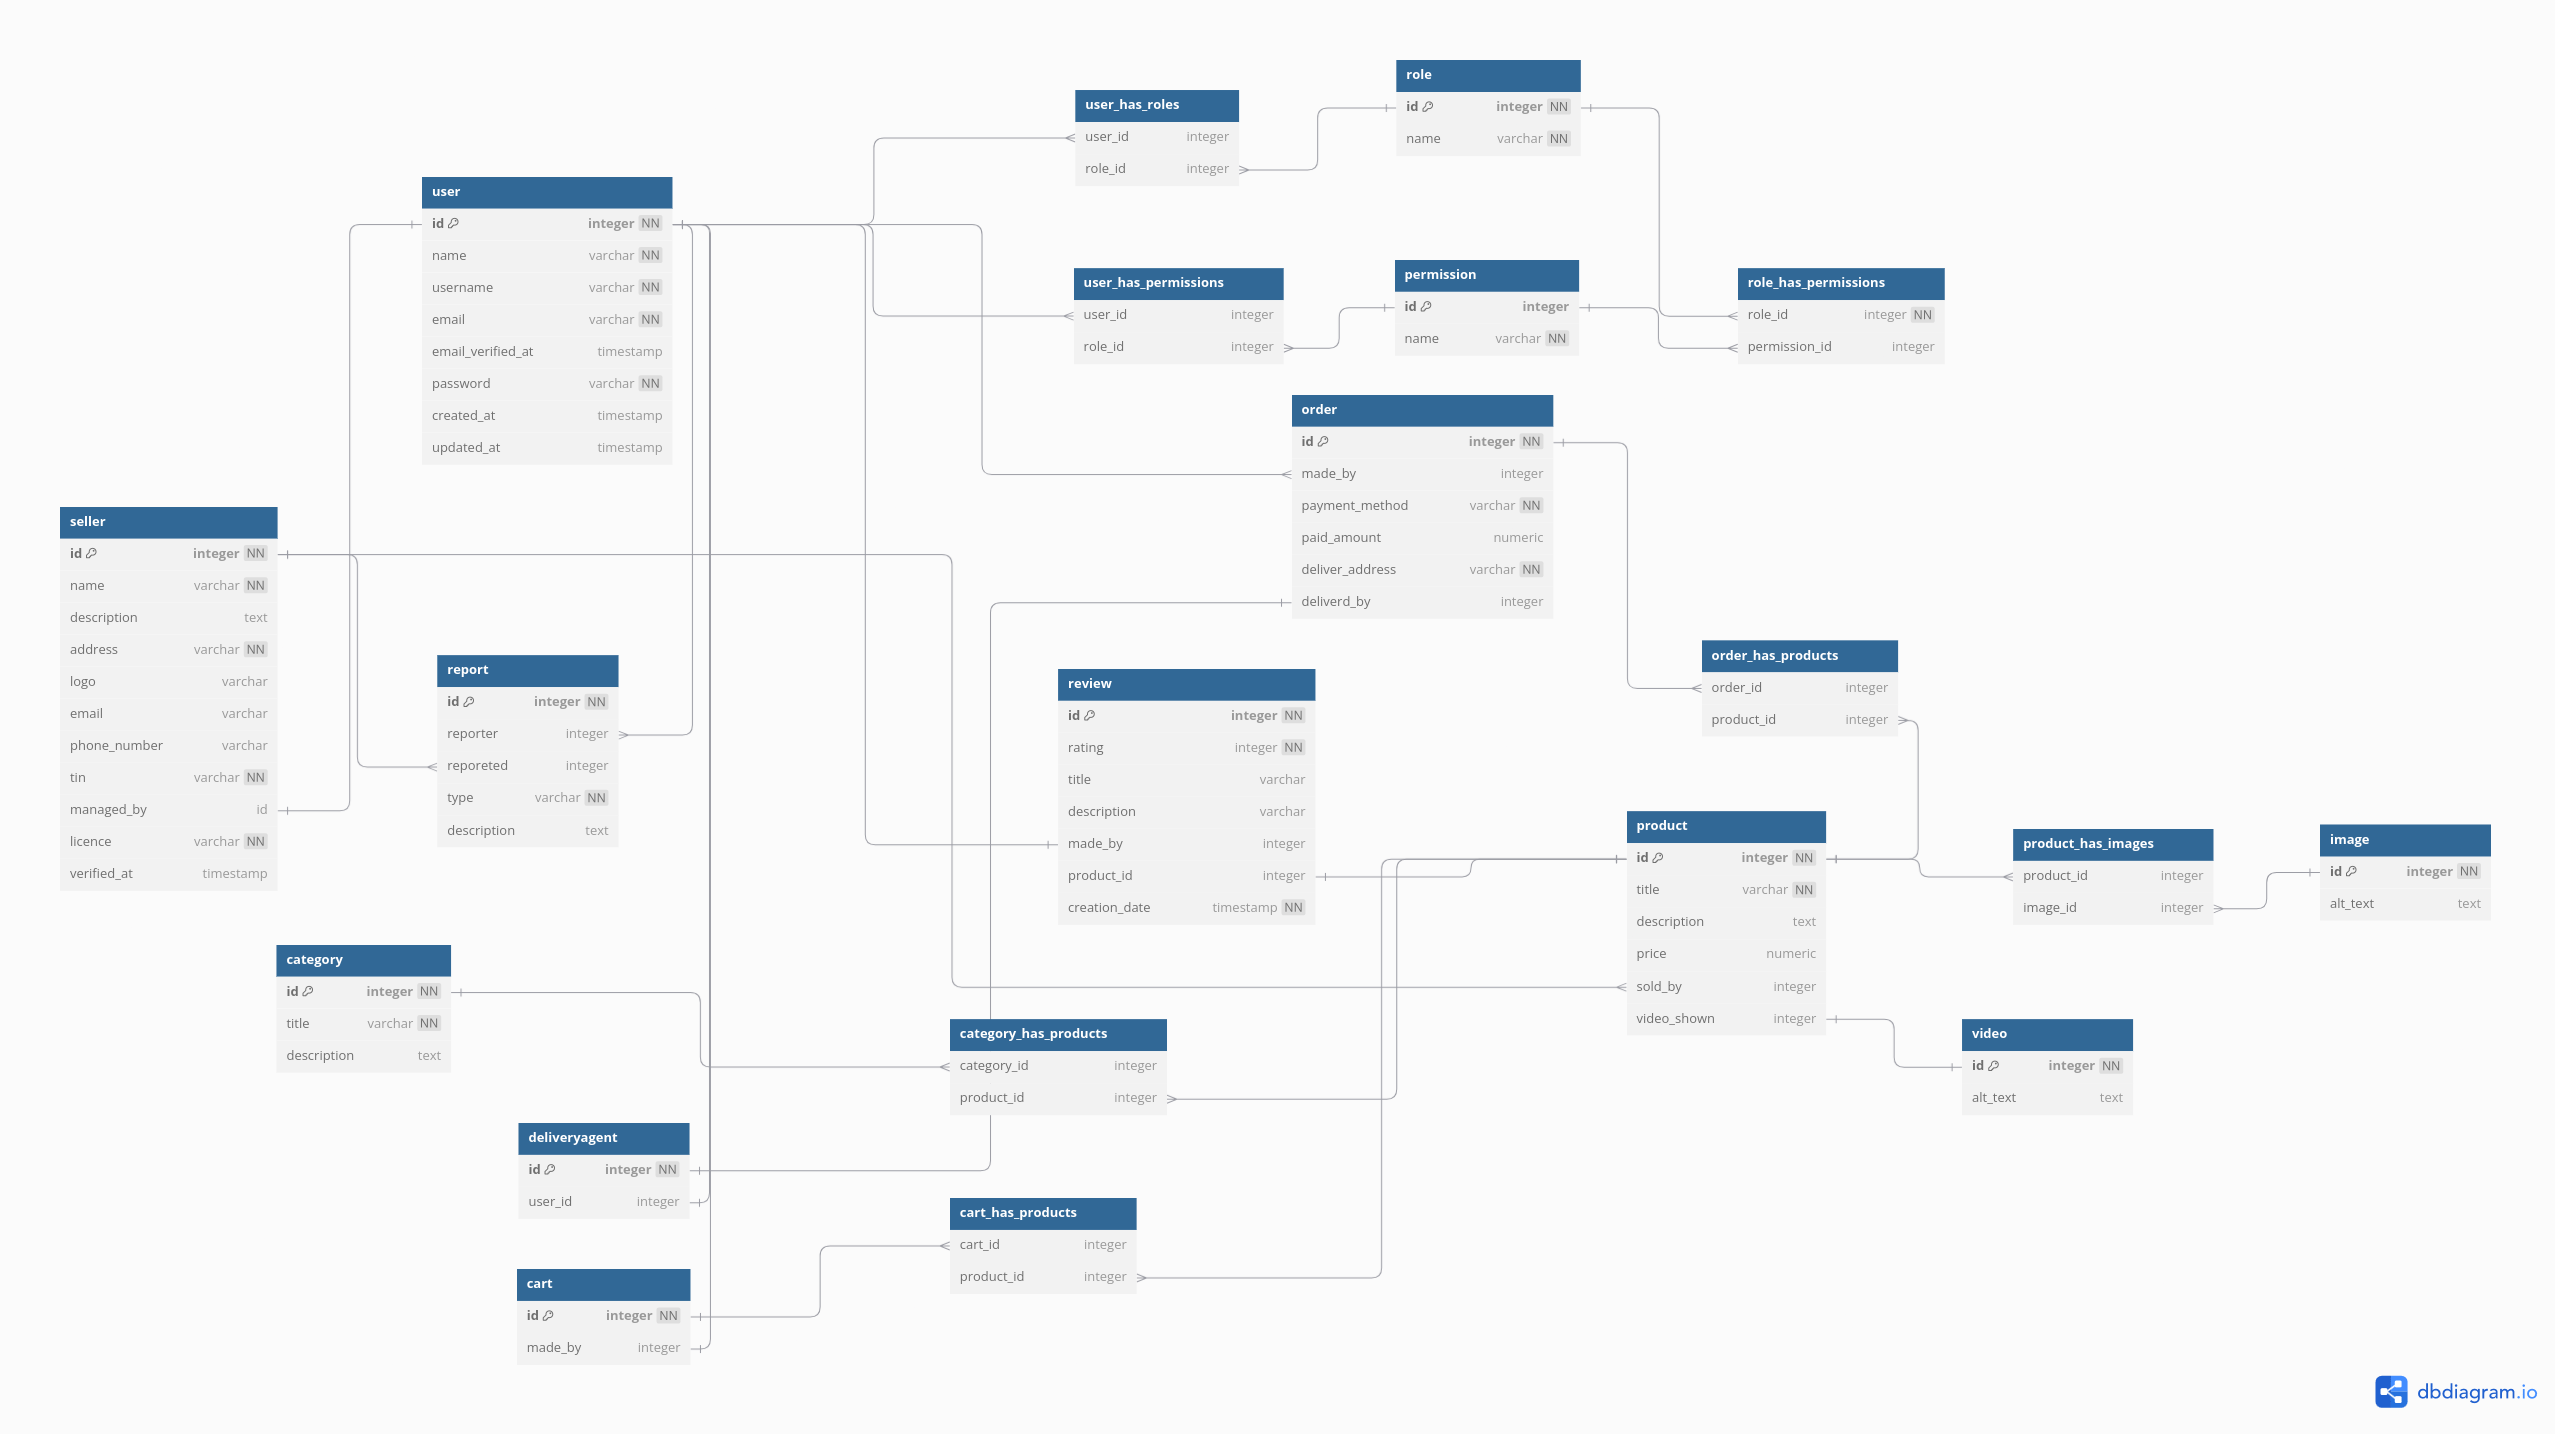
\includegraphics[width=1\textwidth]{diagrams/er}
		\end{center}
		\caption{ER Diagram for PRICO}\label{fig:fig2}
	\end{figure}
\end{frame}

\section{End}
\begin{frame}
	\frametitle{End!}
	\Large
	\centering
	Thank You!
\end{frame}

\end{document}
